\documentclass[letterpaper]{article}
\usepackage{natbib}
\usepackage[utf8]{inputenc}

\usepackage{fullpage,epsf,fancyheadings}
\usepackage{amsmath}
\usepackage{graphicx}
\usepackage{tikz}
\usepackage{amsmath}
\usepackage[toc]{appendix}
\usepackage[frenchb]{babel}
\usepackage[T1]{fontenc}
\usepackage{placeins, latexsym, amssymb}
\usepackage[hidelinks]{hyperref}
\usepackage{url}

\usepackage{listings}
\usepackage{color}

\definecolor{codegreen}{rgb}{0,0.6,0}
\definecolor{codegray}{rgb}{0.5,0.5,0.5}
\definecolor{codepurple}{rgb}{0.58,0,0.82}
\definecolor{backcolour}{rgb}{0.95,0.95,0.92}

\lstdefinestyle{mystyle}{
  backgroundcolor=\color{backcolour},
  commentstyle=\color{codegreen},
  keywordstyle=\color{magenta},
  numberstyle=\tiny\color{codegray},
  stringstyle=\color{codepurple},
  basicstyle=\ttfamily\footnotesize,
  breakatwhitespace=false,
  breaklines=true,
  captionpos=b,
  keepspaces=true,
  numbers=left,
  numbersep=5pt,
  showspaces=false,
  showstringspaces=false,
  showtabs=false,
  tabsize=2
}

\lstset{style=mystyle}


\begin{document}
\begin{titlepage}
  \begin{tikzpicture}[remember picture, overlay]
    \node [anchor=north east, inner sep=0pt]  at (current page.north east)
    {
\includegraphics[height=3cm]{Baniere_ULB.png}};
  \end{tikzpicture}
  \begin{center}
    \textbf{\textsc{UNIVERSIT\'E LIBRE DE BRUXELLES}}\\
    \textbf{\textsc{Faculté des Sciences}}\\
    \textbf{\textsc{Département d'Informatique}}
    \vfill{}\vfill{}
    \begin{center}{\Huge INFO-F-302 Informatique Fondamentale: Rapport de projet}\end{center}{\Huge \par}
    \begin{center}{\large \textsc{Perale} Thomas\\\textsc{Requena} Carlos}\end{center}{\Huge \par}
    \vfill{}\vfill{}
    \vfill{}\vfill{}\enlargethispage{3cm}

    \begin{figure} [h!]
      \centering
      
\includegraphics[width=4cm]{Sigle_ULB.png}
    \end{figure}

    \textbf{Année académique 2016~-~2017}
  \end{center}

\end{titlepage}

\tableofcontents
\pagebreak

\section{Introduction}

Le but du projet est de modéliser des problèmes de satisfaction de contraintes
à l'aide de l'outil de résolution de contraintes \texttt{ChocoSolver}\footnote{http://www.choco-solver.org}. Pour celà
on nous présente plusieurs problèmes en un premier temps basé sur un échiquier
et la modélisation des pièces de celui-ci. En un deuxième temps basé sur la
disposition d'un musée et de l'emplacement que doivent avoir les cameras dans
celui-ci.

\section{Question 1: Le problème d'indépendance}

\subsection{Définition du problème}

Comme il a été dit dans l'énoncé le problème d'indépendance consiste à
déterminer dans un échiquier de taille donné si il est possible d'assigner à
chacune des pièces misent à notre disposition (c'est à dire autant de
chevalier, tour ou fou que l'on veut) une position distincte de sorte qu'aucune
pièce ne menace une autre pièce.

\subsection{Définition des variables}

\begin{itemize}
\item \textit{n} la taille de l'échiquier;
\item \textit{t} le nombre de tour;
\item \textit{f} le nombre de fou;
\item \textit{c} le nombre de chevalier;
\end{itemize}

\subsection{Contraintes}

\begin{itemize}
\item Chaque pièce doit occuper une case diffèrente.

\item Aucune pièce ne peut occuper les cases situées à gauche, à
  droite, en haut et en bas des toutes les tours.
\item Aucune pièce ne peut occuper les cases situées en diagonale des
  tous les fous.
\item Aucune pièce ne peut occuper les cases menacées par tous les
  cavaliers (\ref{fig:cavalier})
\end{itemize}

\begin{figure}[ht]
  \centering
  \label{fig:cavalier}
  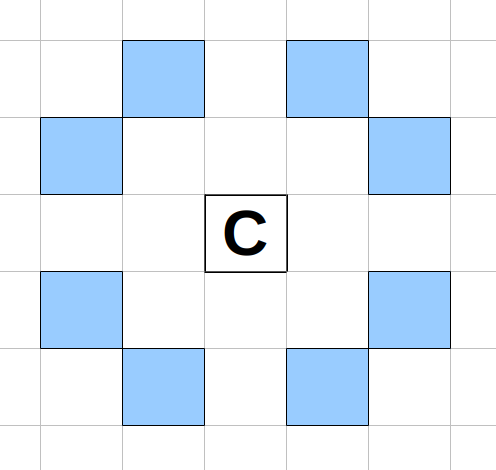
\includegraphics[width=5cm]{fig/cavalier.png}
  \caption{Cases menacées par un cavalier}
\end{figure}

\section{Question 2: Le problème de domination}

\subsection{Définition du problème}

Ce problème cherche à ce que chaque case de l'échiquier doive être soit
occupée soit menacée par au moins une pièce.

\subsection{Définition des variables}

\begin{itemize}
\item \textit{n} la taille de l'échiquier;
\item \textit{t} le nombre de tour;
\item \textit{f} le nombre de fou;
\item \textit{c} le nombre de chevalier;
\end{itemize}

\subsection{Contraintes}

\begin{itemize}
\item Chaque pièce doit occuper une case diffèrente.
\item Toute pièce doit occuper soit:
  \begin{itemize}
  \item les cases situées à gauche, à droite, en haut et en bas des
    toutes les tours.
  \item les cases situées en diagonale des tous les fous.
  \item les cases menacées par tous les cavaliers (\ref{fig:cavalier}).
  \end{itemize}
\end{itemize}


\section{Question 4: Les chevaliers minimum}

\subsection{Définition du problème}

Ce problème calcule le nombre minimal de cavaliers permettant de dominer
un échiquier de taille donné.

Pour résoudre ce problème, il faut changer de tactique avec
ChocoSolver. On ne cherche pas a savoir si une solution existe, mais
plutôt a connaître la quantité minimale de chevaliers nécessaires pour
menacer tout l'échiquier:

\begin{lstlisting}[language=java]
  // to minimise X
  model.setObjectives(Model.MINIMIZE, X);
\end{lstlisting}

\subsection{Définition des variables}

\begin{itemize}
\item \textit{n} la taille de l'échiquier;
\end{itemize}

\subsection{Contraintes}

\begin{itemize}
\item Chaque pièce doit occuper une case diffèrente. Chaque chevalier
  doit occuper une et une seule case libre de l'échiquier.
\item Toutes les cases de l'échiquier doivent menacées par au moins un
  cavalier. C'est à dire, toutes les cases devront être bleues dans la
  figure (\ref{fig:cavalier}), sauf les cases déjà occupées par les cavaliers.
\end{itemize}


\section{Question 5: La surveillance de musée}

Ici le problème est essentiellement le même, appliqué à la
surveillance d'un musée.

\newpage

\appendix

\section{Code Listing}

\lstinputlisting[language=Java]{../src/main/java/chocolatte/App.java}


\end{document}
